%% An Introduction to LaTeX Thesis Template of Wuhan University
%%
%% Created by WHUTUG

\documentclass[type=master, class=academic]{whu-thesis}
\usepackage{rotating}
% 注释掉下面这行编译出来的即为不插入空白页,不注释则为插入空白页
% \renewcommand{\cleardoublepage}{\clearpage}
\newcommand{\figcite}[1]{\scalebox{1.3}[1.3]{\raisebox{-0.7ex}{\cite{#1}}}}
\whusetup
  {
    info               =
      {
        title          = {武汉大学学位论文 \LaTeX{} 模板\\使用示例文档},
        title*         = {An Introduction to LaTeX Thesis Template\\of Wuhan University},
%%%%% ------------------------------------------------------------------- %%%%%
        student-number = {20XX20211XXXX},
        school         = {计算机学院},
        school*        = {School of Computer Science},
        author         = {XXxx},
        author*        = {\sc xx XX},
        clc            = {TP391},%%%%%
        % subject        = {学科},
        major          = {计算机科学与技术},
        major*         = {Computer Science and Technology},
        advisor        = {XXxx , 教授},
        advisor*       = {\sc Prof.~xx XX},
%%%%% -------------------- Upload System ----- BEGIN -------------------- %%%%%
        % student-number = {},
        % school         = {计算机学院},
        % school*        = {School of Computer Science},
        % author         = {},
        % author*        = {},
        % clc            = {TP391},%%%%%
        % % subject        = {学科},
        % major          = {计算机科学与技术},
        % major*         = {Computer Science and Technology},
        % advisor        = {},
        % advisor*       = {},
%%%%% -------------------- Upload System ----- END -------------------- %%%%%
        direction      = {自然语言处理},%%%%
        direction*     = {Natural Language Processing},%%%%
        % date           = {2022/5},
        keywords       = {关键词 1 , 关键词 2 , 关键词 3 , 关键词 4 , 一个非常非常,非常非常长——的关键词 5},
        keywords*      = {key word 1 , key word 2 , key word 3 , key word 4 , {and a very very, very very long key word---the key word 5}},
      },
    style              =
      {
        graphics-path  = {{figures/}{data/}},
        list-of-figures,
        list-of-tables,
        % bib-backend    = {bibtex},
        bib-style      = {numerical},
        cite-style     = {numerical-super},
        cjk-font       = overleaf
      },
    element            =
      {
        innovation     = {pages/innovation},
        abstract       = {pages/abstract},
        abstract*      = {pages/enabstract},
        bibliography   = {ref/refs},
        achievements   = {pages/achievements},
        thanks         = {pages/thanks},
        appendix       = {pages/appendix}
      }
  }

\begin{document}
%%----------- 主体部分 ----------- %%
\include{pages/chapter1}
\include{pages/chapter2}
% Chapter 3

\chapter{引用与链接}

\section{脚注}
注释是对论文中特定名词或新名词的注解。注释可用页末注或篇末注的一种。选择页末注的应在注释与正文之间加细线分隔,线宽度为 1 点,线的长度不应超过纸张的三分之一宽度。同一页类列出多个注释的,应根据注释的先后顺序编排序号。字体为宋体5号,注释序号以“\circled{1}、\circled{2}”等数字形式标示在被注释词条的右上角。页末或篇末注释条目的序号应按照“\circled{1}、\circled{2}”等数字形式与被注释词条保持一致,脚注序号每面更新。示例:这里有个注释\footnote{我是解释注释的}。

\section{引用文中小节}\label{sec:ref}
如引用小节~\ref{sec:ref}

\section{引用参考文献}
这是一个参考文献引用的范例:BERT(Bidirectional Encoder Representations from Transformers)模型 \cite{devlin2018bert} 是由 Google AI 团队与 2018 年提出的语言表示模型,发布时在 NLP 领域的 11 个任务上取得了最好结果。经过微调后, BERT 可以灵活的应用在下游人物中。更多引用命令请参阅 natbib 文档或 biblatex 文档。\nocite{*}

文献引用需要配合 BibTeX 使用,很多工具可以直接生成 BibTeX 文件(如 EndNote、NoteExpress、百度学术、谷歌学术等),此处不作介绍。

\section{图片引用}

\begin{figure}[htbp]
    \centering
    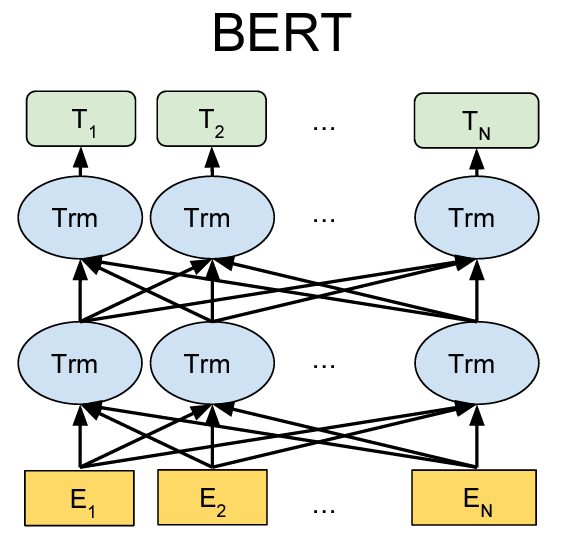
\includegraphics[width=0.3\textwidth]{figures/bert.png}
    \caption{BERT 模型结构}
    \label{fig:bert}
\end{figure}

图片引用可以使用 \verb|\figcite{}|,如:BERT 模型结构图如图 ~\ref{fig:bert}(图片来源:文献\figcite{devlin2018bert}) 所示。

\section{链接相关}
模板使用了 hyperref 包处理相关链接,使用 \verb|\href| 可以生成超链接,默认不显示链接颜色。如果需要输出网址,可以使用 \verb|\url| 命令,示例:\url{https://github.com}。
\include{pages/chapter4}
% Chapter 5

\chapter{实验与分析}

% Chapter 6

\chapter{全文总结与展望}



\end{document}